\documentclass[12pt]{article}
\usepackage[left=1cm, right=1cm, top=2cm,bottom=1.5cm]{geometry} 

\usepackage[parfill]{parskip}
\usepackage[utf8]{inputenc}
\usepackage[T2A]{fontenc}
\usepackage[russian]{babel}
\usepackage{enumitem}
\usepackage[normalem]{ulem}
\usepackage{amsfonts, amsmath, amsthm, amssymb, mathtools,xcolor}
\usepackage{blkarray}

\usepackage{tabularx}
\usepackage{hhline}

\usepackage{accents}
\usepackage{fancyhdr}
\pagestyle{fancy}
\renewcommand{\headrulewidth}{1.5pt}
\renewcommand{\footrulewidth}{1pt}

\usepackage{graphicx}
\usepackage[figurename=Рис.]{caption}
\usepackage{subcaption}
\usepackage{float}

%%Наименование папки откуда забирать изображения
\graphicspath{ {./images/} }

%%Изменение формата для ввода доказательства
\renewcommand{\proofname}{$\square$  \nopunct}
\renewcommand\qedsymbol{$\blacksquare$}

%%Изменение отступа на таблицах
\addto\captionsrussian{%
	\renewcommand{\proofname}{$\square$ \nopunct}%
}
%% Римские цифры
\newcommand{\RN}[1]{%
	\textup{\uppercase\expandafter{\romannumeral#1}}%
}

%% Для удобства записи
\newcommand{\MR}{\mathbb{R}}
\newcommand{\MC}{\mathbb{C}}
\newcommand{\MQ}{\mathbb{Q}}
\newcommand{\MN}{\mathbb{N}}
\newcommand{\MZ}{\mathbb{Z}}
\newcommand{\MTB}{\mathbb{T}}
\newcommand{\MTI}{\mathbb{I}}
\newcommand{\MI}{\mathrm{I}}
\newcommand{\MCI}{\mathcal{I}}
\newcommand{\MJ}{\mathrm{J}}
\newcommand{\MH}{\mathrm{H}}
\newcommand{\MT}{\mathrm{T}}
\newcommand{\MU}{\mathcal{U}}
\newcommand{\MV}{\mathcal{V}}
\newcommand{\MB}{\mathcal{B}}
\newcommand{\MF}{\mathcal{F}}
\newcommand{\MW}{\mathcal{W}}
\newcommand{\ML}{\mathcal{L}}
\newcommand{\MP}{\mathcal{P}}
\newcommand{\VN}{\varnothing}
\newcommand{\VE}{\varepsilon}
\newcommand{\dx}{\, dx}
\newcommand{\dy}{\, dy}
\newcommand{\dz}{\, dz}
\newcommand{\dd}{\, d}


\theoremstyle{definition}
\newtheorem{defn}{Опр:}
\newtheorem{rem}{Rm:}
\newtheorem{prop}{Утв.}
\newtheorem{exrc}{Упр.}
\newtheorem{problem}{Задача}
\newtheorem{lemma}{Лемма}
\newtheorem{theorem}{Теорема}
\newtheorem{corollary}{Следствие}

\newenvironment{cusdefn}[1]
{\renewcommand\thedefn{#1}\defn}
{\enddefn}

\DeclareRobustCommand{\divby}{%
	\mathrel{\text{\vbox{\baselineskip.65ex\lineskiplimit0pt\hbox{.}\hbox{.}\hbox{.}}}}%
}
\DeclareRobustCommand{\ndivby}{\mkern-1mu\not\mathrel{\mkern4.5mu\divby}\mkern1mu}


%Короткий минус
\DeclareMathSymbol{\SMN}{\mathbin}{AMSa}{"39}
%Длинная шапка
\newcommand{\overbar}[1]{\mkern 1.5mu\overline{\mkern-1.5mu#1\mkern-1.5mu}\mkern 1.5mu}
%Функция знака
\DeclareMathOperator{\sgn}{sgn}

%Функция ранга
\DeclareMathOperator{\rk}{\text{rk}}
\DeclareMathOperator{\diam}{\text{diam}}


%Обозначение константы
\DeclareMathOperator{\const}{\text{const}}

\DeclareMathOperator{\codim}{\text{codim}}

\DeclareMathOperator*{\dsum}{\displaystyle\sum}
\newcommand{\ddsum}[2]{\displaystyle\sum\limits_{#1}^{#2}}

%Интеграл в большом формате
\DeclareMathOperator{\dint}{\displaystyle\int}
\newcommand{\ddint}[2]{\displaystyle\int\limits_{#1}^{#2}}
\newcommand{\ssum}[1]{\displaystyle \sum\limits_{n=1}^{\infty}{#1}_n}

\newcommand{\smallerrel}[1]{\mathrel{\mathpalette\smallerrelaux{#1}}}
\newcommand{\smallerrelaux}[2]{\raisebox{.1ex}{\scalebox{.75}{$#1#2$}}}

\newcommand{\smallin}{\smallerrel{\in}}
\newcommand{\smallnotin}{\smallerrel{\notin}}

\newcommand*{\medcap}{\mathbin{\scalebox{1.25}{\ensuremath{\cap}}}}%
\newcommand*{\medcup}{\mathbin{\scalebox{1.25}{\ensuremath{\cup}}}}%

\makeatletter
\newcommand{\vast}{\bBigg@{3.5}}
\newcommand{\Vast}{\bBigg@{5}}
\makeatother

%Промежуточное значение для sup\inf, поскольку они имеют разную высоту
\newcommand{\newsup}{\mathop{\smash{\mathrm{sup}}}}
\newcommand{\newinf}{\mathop{\mathrm{inf}\vphantom{\mathrm{sup}}}}

%Скалярное произведение
\newcommand{\inner}[2]{\left\langle #1, #2 \right\rangle }
\newcommand{\linsp}[1]{\left\langle #1 \right\rangle }
\newcommand{\linmer}[2]{\left\langle #1 \vert #2\right\rangle }

%Подпись символов снизу
\newcommand{\ubar}[1]{\underaccent{\bar}{#1}}

%% Шапка для букв сверху
\newcommand{\wte}[1]{\widetilde{#1}}
\newcommand{\wht}[1]{\widehat{#1}}
\newcommand{\ovl}[1]{\overline{#1}}

%%Трансформация Фурье
\newcommand{\fourt}[1]{\mathcal{F}\left(#1\right)}
\newcommand{\ifourt}[1]{\mathcal{F}^{-1}\left(#1\right)}

%%Символ вектора
\newcommand{\vecm}[1]{\overrightarrow{#1\,}}

%%Пространстов матриц
\newcommand{\matsq}[1]{\operatorname{Mat}_{#1}}
\newcommand{\mat}[2]{\operatorname{Mat}_{#1, #2}}

%Оператор для действ и мнимых чисел
\DeclareMathOperator{\IM}{\operatorname{Im}}
\DeclareMathOperator{\RE}{\operatorname{Re}}
\DeclareMathOperator{\li}{\operatorname{li}}
\DeclareMathOperator{\GL}{\operatorname{GL}}
\DeclareMathOperator{\SL}{\operatorname{SL}}
\DeclareMathOperator{\Char}{\operatorname{char}}
\DeclareMathOperator\Arg{Arg}

%Делимость чисел
\newcommand{\modn}[3]{#1 \equiv #2 \; (\bmod \; #3)}


%%Взятие в скобки, модули и норму
\newcommand{\parfit}[1]{\left( #1 \right)}
\newcommand{\modfit}[1]{\left| #1 \right|}
\newcommand{\sqparfit}[1]{\left\{ #1 \right\}}
\newcommand{\normfit}[1]{\left\| #1 \right\|}

%%Функция для обозначения равномерной сходимости по множеству
\newcommand{\uconv}[1]{\overset{#1}{\rightrightarrows}}
\newcommand{\uconvm}[2]{\overset{#1}{\underset{#2}{\rightrightarrows}}}


%%Функция для обозначения нижнего и верхнего интегралов
\def\upint{\mathchoice%
	{\mkern13mu\overline{\vphantom{\intop}\mkern7mu}\mkern-20mu}%
	{\mkern7mu\overline{\vphantom{\intop}\mkern7mu}\mkern-14mu}%
	{\mkern7mu\overline{\vphantom{\intop}\mkern7mu}\mkern-14mu}%
	{\mkern7mu\overline{\vphantom{\intop}\mkern7mu}\mkern-14mu}%
	\int}
\def\lowint{\mkern3mu\underline{\vphantom{\intop}\mkern7mu}\mkern-10mu\int}

%%След матрицы
\DeclareMathOperator*{\tr}{tr}

\makeatletter
\renewcommand*\env@matrix[1][*\c@MaxMatrixCols c]{%
	\hskip -\arraycolsep
	\let\@ifnextchar\new@ifnextchar
	\array{#1}}
\makeatother


%% Переопределение функции хи, чтобы выглядела более приятно
\makeatletter
\@ifdefinable\@latex@chi{\let\@latex@chi\chi}
\renewcommand*\chi{{\@latex@chi\smash[t]{\mathstrut}}} % want only bottom half of \mathstrut
\makeatletter

\setcounter{MaxMatrixCols}{20}

\begin{document}
\lhead{Алгебра-\RN{1}}
\chead{Тимашев Д.А.}
\rhead{Лекция - 19}
\section*{Неприводимые многочлены над $\MQ$}
Классификация многочленов над $\MQ$ - сложная задача. 

\textbf{Факт}: $x^n + 2$ - неприводим над $\MQ, \, \forall n \geq 2$. Это следует из критерия Эйзенштейна и будет рассмотрен в $3$-м семестре.

\begin{theorem}
	Пусть $f(x) \in \MZ[x]$, то есть: 
	$$
		f(x) = a_n x^n + \dotsc + a_1 x + a_0, \, a_i \in \MZ
	$$ 
	Тогда $x = \dfrac{u}{v}, \, u,v \in \MZ, \, (u,v) = 1$ является корнем $f(x) \Rightarrow a_n \divby v, \, a_0 \divby v$.
\end{theorem}
\begin{proof}
	$$
		0 = a_n{\cdot}\dfrac{u^n}{v^n} + \dotsc + a_1{\cdot}\dfrac{u}{v} + a_0 \Rightarrow 0 = \underbrace{a_n u^n + \dotsc + a_1 u v^{n-1}}_{\text{делится на } u}+ a_0 v^n \Rightarrow
	$$
	$$
		\Rightarrow -a_0v^n = a_n u^n + \dotsc + a_1 u v^{n-1} \divby u \Rightarrow -a_0v^n \divby u, \, (u,v) = 1 \Rightarrow (u,v^n) = 1
	$$
	По аналогии:
	$$
		0 = a_nu^n + \underbrace{a_{n-1}u^{n-1}v + \dotsc + a_1 v u^{n-1} + a_0v^n}_{\text{делится на }v} \Rightarrow a_nu^n \divby v \Rightarrow a_n \divby v
	$$
\end{proof}
\begin{corollary}(\textbf{Алгоритм нахождения всех корней $f(x) \in Q[x]$})
	\begin{enumerate}[label=\arabic*)]
		\item $f(x) \in \MQ[x] \Rightarrow g(x) \in \MZ[x]$ - перейти от многочлена $\in \MQ[x]$ к многочлену $\in \MZ[x]$, домножив на НОК знаменателей рациональных коэффициентов. Понятно, что корни от этого не изменятся;
		\item Перебрать все пары $(u,v) \colon a_0 \divby u, \, a_n \divby v$. Можно считать, что $a_0 \neq 0, \, a_n \neq 0$. $a_n \neq 0$ как старший член. Если $a_0 = 0$, то $0$ является корнем. Разделив уравнение на $x$ в подходящей степени, получим уравнение с ненулевым свободным членом, либо корнями уравнения будут только нули. Множество делителей $a_n$ и $a_0$ конечно $\Rightarrow$ количество пар $(u,v)$ конечно;
		
		\item Подставляем все $\dfrac{u}{v}$ в $g(x)$ и находим корни;
		
		\item (Схема Горнера) Находим кратности полученных корней;
	\end{enumerate}
\end{corollary}

\begin{rem}
	Заметим, что если мы нашли корни многочлена, это ещё не значит, что он распался на линейные множители. Возможно в разложении будет присутствовать множитель, который корней над данным полем не имеет.
\end{rem}

\textbf{Факт}: Существует алгоритм Дедекинда разложения многочлена $f(x) \in \MQ[x]$ на неприводимые множители над $\MQ$. 

Теорема выше - часть этого алгоритма, позволяющего найти линейные множители разложения. Оставшуюся часть также нужно разложить на неприводимые множители более высоких степеней и алгоритм Дедекинда описывает этот процесс.

\newpage
\section*{Нахождение корней многочленов над полем $\MR$}
Мы видели, что разложение многочлена на неприводимые множители над $\MR$ или $\MC$ сводится к нахождению его комплексных корней. Отметим, что явных формул для выражения корней многочленов, которые выражают корни этих многочленов через их коэффициенты с помощью каких-то операций сложения, умножения, деления, извлечения корней не существует для многочленов степени выше $4$.
\begin{theorem}(\textbf{Руффини-Абеля})
	Общее уравнение степени $\geq 5$ не разрешимо в радикалах.
\end{theorem}
Термин общее уравнение здесь мы будем понимать как обычный многочлен степени $n$.

Вопрос о нахождении корней заданного многочлена, часто сводится к тому, что важны не точные значения корней, а приближенные. То есть нужно уметь находить корни многочлена приближенно со сколь угодно заданной точностью. Для этого достаточно уметь находить количество корней заданного многочлена в заданном интервале (для $\MR$)/заданной области комплексной плоскости (для $\MC$).

\subsection*{Приближенное нахождение корней многочлена на заданном интервале}
Пусть у нас есть некий многочлен $f \in \MR[x]$ и мы умеем искать количество корней на любом интервале. У нас есть интервал и некоторое количество корней многочлена $f$ на нем. Мы хотим найти эти корни со сколь угодно заданной точностью. Предположим, что мы посчитали общее количество корней на этом интервале, нашли сколько их и поделили интервал пополам. Затем посчитали сколько корней на каждой половине. Затем поделили каждую из половин ещё на две равные части и посчитали количество корней уже на них. Продолжаем эту процедуру.
\begin{figure}[H]
	\centering
	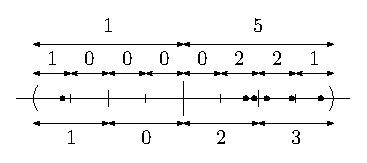
\includegraphics[width=0.35\textwidth]{AL1L19_1.eps}
	\caption{Поиск корней на заданном интервале.}
	\label{19_1}
\end{figure}
Рано или поздно, мы каждый из корней окружим таким маленьким интервалом, внутри которого он будет содержаться (только один корень) так, что мы найдем его со сколь угодно заданной точностью. Если мы умеем искать количество корней в любой области $\MC$, то рассуждая точно также, мы можем эти корни локализовать - заключить в окрестности со сколь угодно малым радиусом.
\begin{figure}[H]
	\centering
	\includegraphics[width=0.25\textwidth]{AL1L19_2.eps}
	\caption{Поиск корней на заданной плоскости.}
	\label{19_2}
\end{figure}

\subsection*{Нахождение количества корней в интервале ($\MR$) или области ($\MC$)}
Есть несколько точных методов нахождения количества корней заданного многочлена на заданном интервале или на заданной области $\MC$. Например, есть метод Штурма, метод подсчета изменения аргумента на $\MC$. Но они обычно требуют достаточно большых вычислений. Мы разберём метод, который дает оценку сверху для $f\in \MR[x]$ и не требует каких-либо вычислений. Пусть: 
$$
	f \in \MR[x], \, f(x) = a_0 + a_1x + \dotsc + a_n x^n
$$ 
Рассмотрим последовательность коэффициентов этого многочлена: $(a_0, a_1,\dotsc, a_n)$. 
\begin{defn}
	Скажем, что в члене $a_k$ последовательности $(a_0, a_1,\dotsc, a_n)$ имеет место \uwave{перемена знака}, если:
	$$
		\exists \, l < k \colon a_k, a_l \neq 0, \, \sgn(a_k) \neq \sgn(a_l), \, a_{l+1} = a_{l+2} = a_{k-1} = 0
	$$ 
\end{defn}
Таким образом, перемена знака происходит, когда последовательность коэффициентов имеет вид:
$$
	a_0, a_1,\dotsc, \underset{\pm}{a_l}, 0, \dotsc, 0, \underset{\mp}{a_k}, \dotsc,  a_n
$$
\textbf{\uline{Обозначение}}: $L(f)$ - число перемен знака в последовательности коэффициентов $(a_0, a_1,\dotsc, a_n)$, без учета нулей.

\textbf{Пример}: $f(x) = 2 + 3x - 5x^3 + 4x^4 + x^6 - 6x^7$, тогда: $L(f) = 3$: $3 \rightarrow -5 \rightarrow 4, \, 1 \rightarrow -6$.

\textbf{\uline{Обозначение}}: $N(f)$ - число \uline{положительных} корней многочлена $f$ с учётом их кратностей.

\begin{theorem}(\textbf{Декарт})
	\begin{enumerate}[label=\arabic*)]
		\item $N(f) \leq L(f)$, причем равенство достигается, если $f$ - не имеет мнимых корней;
		\item $\modn{N(f)}{L(f)}{2}$, то есть четность $N(f)$ такая же, как у $L(f)$;
	\end{enumerate}
\end{theorem}
\begin{rem}
	Другое название теоремы Декарта - \textbf{правило знаков}.
\end{rem}
\begin{proof}\hfill
	\begin{enumerate}[label=(\arabic*)]
		\item Пусть $a_n \neq 0, \, \deg(f) = n$. Заменив $f$ на $-f$ при необходимости, можно считать, что $a_n > 0$, при этом число положительных корней и число перемен знаков последовательности коэффициентов при такой замене не изменится. Поэтому доказав с этим условием, мы докажем и $\forall f \in \MR[x]$. Тогда:
		$$
			f(x) = a_kx^k  + \dotsc + a_n x^n, \, a_k \neq 0, \, a_n > 0
		$$
		где $a_k$ - первый ненулевой коэффициент;
		
		\item Поделим $f$ на $x^k \Rightarrow$ можем считать, что $a_0 \neq 0$ и $n - k = n$. Число положительных корней не изменится, поскольку нулевые корни нас не интересуют. Число перемен знака тоже не изменится, поскольку в последовательности коэффициентов мы просто отрезаем кусок из нулей. Тогда:
		$$
			f(x) = a_0 + \dotsc + a_{n}x^{n}, \, a_0 \neq 0, \, a_{n} > 0
		$$
		Пусть: $x_1 < x_2 < \dotsc < x_s$ - все $+$ корни $f$. Обозначим их кратности: $k_1, k_2,\dotsc, k_s$;
		\begin{figure}[H]
			\centering
			\includegraphics[width=0.4\textwidth]{AL1L19_3.eps}
			\caption{Многочлен $f(x)$ и его корни: $x_1 < x_2 < \dotsc < x_s$.}
			\label{19_3}
		\end{figure}
		\item Докажем, что $\modn{N(f)}{L(f)}{2}$. Рассмотрим $\sgn f(x)$ при изменении $x$ от $0$ до $+\infty$:
		\begin{enumerate}[label=\alph*)]
			\item $x_i < x < x_{i+1} \Rightarrow \sgn f(x) = \const \Rightarrow$ надо смотреть, что происходит при переходе через корень многочлена; 
			\item Рассмотрим произвольный корень $x_i$ кратности $k_i$, тогда:
			$$
				f(x) = (x - x_i)^{k_i}{\cdot}g(x), \, g(x_i) \neq 0
			$$
			Следовательно, в окрестности точки $x_i$ многочлен $g(x)$ имеет тот же самый знак, что и в точке $g(x_i) \neq 0$. Сдвигаясь вправо, получим:
			$$
				x_i < x < x_i + \VE \Rightarrow x - x_i > 0 \Rightarrow \sgn f(x) = \sgn g(x_i)
			$$
			Сдвигаясь левее, получим:
			$$
				x_i - \VE < x < x_i \Rightarrow x - x_i < 0 \Rightarrow \sgn f(x) = (-1)^{k_i}{\cdot}\sgn g(x_i)
			$$
			Если $k_i$ - четное, то знак не поменяется, если нечетно, то знак поменяется;
			\item При $0 < x < \VE \Rightarrow \sgn f(x) = \sgn a_0$;
			\item При $x \to +\infty$, вынесем $x^n$, тогда многочлен $f(x)$ приобретет вид:
			$$
				f(x) = x^n{\cdot}\left(\dfrac{a_0}{x^n} + \dfrac{a_1}{x^{n-1}} + \dotsc + \dfrac{a_{n-1}}{x} + a_n\right) \Rightarrow \dfrac{a_0}{x^n} + \dfrac{a_1}{x^{n-1}} + \dotsc + \dfrac{a_{n-1}}{x} + a_n \xrightarrow[x \to +\infty]{} a_n
			$$
			Поскольку $a_n > 0, \, x > 0$, тогда:
			$$
				\exists \, C > 0, \, \forall x > C \Rightarrow \sgn f(x) = \sgn a_n > 0
			$$
		\end{enumerate}
		Таким образом, при прохождении через корень кратности $k$, $\sgn f(x)$ меняется $k$ раз $\Rightarrow$ 
		общее количество перемен знака $=$ числу положительных корней, с учётом кратности. Если сумма кратных корней - чётна, то знак меняется четное число раз и не изменится при переходе от $0$ к $+\infty$:
		$$
			N(f) = k_1 + k_2 + \dotsc + k_s = 2m, \, m \in \MN, \, a_n > 0 \Rightarrow a_0 > 0
		$$
		Если коэффициенты $a_0 > 0, \, a_n > 0 \Rightarrow L(f)$ - чётно:
		$$
			(\underset{+}{a_0}, \dotsc, \underset{+}{a_n}) \Rightarrow L(f) = 2k, \, k \in \MN
		$$
		Если сумма кратных корней - нечётна, то:
		$$
			N(f) = k_1 + k_2 + \dotsc + k_s = 2m + 1, \, m \in \MN, \, a_n > 0 \Rightarrow a_0 < 0
		$$	
		аналогично, поскольку знак при переходе от $0$ к $+\infty$ не меняется $\Rightarrow L(f)$ - нечётно:
		$$
			(\underset{-}{a_0}, \dotsc, \underset{+}{a_n})  \Rightarrow L(f) = 2k + 1, \, k \in \MN
		$$
		Следовательно: $\modn{N(f)}{L(f)}{2}$ и пункт $2)$ - доказан;
		\item Докажем, что $N(f') \geq N(f) -1$. Положительные корни многочлена бывают простые и кратные. Если кратность корня $x_i$ равна $k_i \geq 2$, то $x_i$ является корнем $f'$, причем кратности $k_i -1$. Если же кратность корня $k_i = 1$, то $x_i$ - не корень $f'$ (или корень кратности $0$). 
		
		Вспомним из анализа \textbf{теорему Ролля}: если в двух крайних точках отрезка значения функции одинаковы, то где-то посередине существует корень из производной. В частности, между любыми двумя соседними корнями нашего многочлена есть корень производной.
		\begin{figure}[H]
			\centering
			\includegraphics[width=0.4\textwidth]{AL1L19_4.eps}
			\caption{Применение теоремы Ролля для нахождения корней производной многочлена $f$.}
			\label{19_4}
		\end{figure}
		Таким образом, по теореме Ролля:
		$$
			\exists \, y_i \in \MR, \, x_i < y_i < x_{i+1} \colon f'(y_i) = 0
		$$
		Следовательно, число корней производной многочлена как минимум будет не меньше суммы кратностей корней исходного многочлена, уменьшеных на единицу плюс число корней между корнями исходного многочлена: 
		$$
			N(f') \geq (k_1 - 1) + (k_2 - 1) + \dotsc + (k_s - 1) + s - 1 = k_1 + k_2 + \dotsc + k_s - s + s -1  = N(f) -1
		$$  
		где $s - 1$ - число корней $f'$ между двумя соседними корня многочлена $f$, тогда:
		\item Докажем, что $L(f') \leq L(f)$. Рассмотрим последовательность коэффициентов $f$:
		$$
			(a_0,a_1,a_2, \dotsc, a_n)
		$$
		Последовательность коэффициентов $f'$ будет иметь вид:
		$$
			(a_1, 2a_2, 3a_3, \dotsc, n a_n)
		$$
		С точностью до положительных множителей, это будут коэффициенты исходного многочлена, без учета первого члена $a_0 \Rightarrow$ число перемен знака в $(a_1,\dotsc, a_n)$ равно $L(f') \Rightarrow$ может возникнуть максимум одна перемена знака $\Rightarrow L(f) \geq L(f')$;
		\item Докажем, что $N(f) \leq L(f)$. Будем доказывать индукцией по $n$:
		
		\uline{База индукции}: $n = 0 \Rightarrow f(x) = a_0 = \const \Rightarrow N(f) = 0, \, L(f) = 0$.
		
		\uline{Шаг индукции}: Воспользуемся пунктом $(4)$: $N(f) \leq N(f') +1 \leq L(f') + 1$ - по предположению индукции. Тогда по $(5)$:
		$$
			N(f) \leq L(f') + 1 \leq L(f) + 1 \wedge \modn{N(f)}{L(f)}{2} \Rightarrow N(f) \neq L(f) + 1 \Rightarrow N(f) \leq L(f)
		$$
		\item Пусть $\wte{f}(x) = f(-x)$, тогда:
		$$
			\wte{f}(x) = a_0 - a_1x + a_2 x^2 - a_3x^3 + \dotsc + (-1)^n{\cdot}a_nx^n
		$$
		Покажем, что $L(f) + L(\wte{f}) \leq n$. Если $a_k \neq 0, \, \forall k$, то на каждом $k$-ом месте ($k = 1,2,\dotsc,n$) есть перемена знака либо в последовательности:
		$$
			(a_0, \dotsc, a_{k-1},a_k,\dotsc, a_n)
		$$
		либо в последовательности:
		$$
			(a_0, \dotsc, (-1)^{k-1}a_{k-1}, (-1)^ka_k, \dotsc, (-1)^na_n)
		$$
		Следовательно, суммарная перемена знака: $L(f) + L(f') = n$. В общем случае, если есть нулевые коэффициенты, то заменим эти $a_k = 0$ на  ненулевые $\Rightarrow L(f)$ и $L(f')$ могут только возрасти и после замены в сумме они станут равны $n$, а до неё они не больше $n$;
		\item Число отрицательных корней $f =$ числу положительных корней $\wte{f}$:
		$$
			f(x_k) = 0, \, x_k > 0 \Leftrightarrow \wte{f}(-x_k) = f(x_k) = 0, \, -x_k < 0 
		$$ 
		\item Если $f$ не имеет мнимых корней $\Rightarrow N(f) + N(\wte{f}) = n$. $x = 0$ - не является корнем, поскольку свободный член не равен $0$. По $(6)$ и $(7)$ мы доказали:
		$$
			N(f) \leq L(f)\wedge N(\wte{f}) \leq L(\wte{f}) \Rightarrow n = N(f) + N(\wte{f}) \leq L(f) + L(\wte{f}) \leq n \Rightarrow 
		$$
		$$
			\Rightarrow N(f) + N(\wte{f}) = \leq L(f) + L(\wte{f}) = n \Rightarrow N(f) = L(f)
		$$
	\end{enumerate}
\end{proof}

\textbf{\uline{Дополнение к правилу знаков}}:
\begin{enumerate}[label=\arabic*)]
	\item Число отрицательных корней многочлена $f = N(\wte{f}) \leq$ числа перемен знаков в последовательности:
	$$
		(a_0, -a_1, a_2, -a_3, \dotsc, (-1)^na_n)
	$$
	то есть, с помощью правила Декарта мы можем оценть сверху количество отрицательных корней многочлена $f$;
	\item Разложим многочлен $f$ по степеням $x - x_0$:
	$$
		f(x) = c_0 + c_1(x - x_0) + \dotsc + c_n(x - x_0)^n
	$$
	Число корней $f$, которые больше, чем $x_0 = N(f)_{>x_0}\leq L(f)_{> x_0} =$ число перемен знаков в последовательности:
	$$
		(c_0, c_1, \dotsc, c_n)
	$$
	или в последовательности:
	$$
		(f(x_0), f'(x_0), \dotsc, f^{(n)}(x_0))
	$$
	поскольку коэффициенты $c_i$ связаны с $f^{(i)}(x_0)$ множителями, которые на знак не влияют. По этой же причине: $\modn{N(f)_{>x_0}}{L(f)_{> x_0}}{2}$. Аналогично, с помощью $1)$ оценивается число корней, которые меньше $x_0$; 
\end{enumerate}
\begin{exrc}
	Найти все действительные корни многочлена: $f(x) = x^4 - x^3 + x^2 - x - 1$ с точностью до знаков после запятой (с точностью до целых чисел).
\end{exrc}

\begin{rem}
	Правило знаков не позволяет отличать простые корни от кратных.
	\begin{figure}[H]
		\centering
		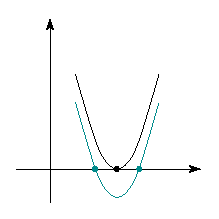
\includegraphics[width=0.3\textwidth]{AL1L19_5.eps}
		\caption{Кратный корень не отличим от простого.}
		\label{19_5}
	\end{figure}
	Два случая на картинке неотличимы друг от друга методом Декарта. Один двухкратный посчитается также, как два однократных, а хотелось бы различать.
\end{rem}
\begin{defn}
	\uwave{Приведенным многочленом} $f_{red}$ многочлена $f$ называется многочлен: $f_{red} = \dfrac{f}{(f,f')}$.
\end{defn}
\begin{prop}
	Пусть $\Char{K} = 0$ и $f \in K[x]$. Тогда $f_{red}$ имеет те же корни, что и $f$, но все корни $f_{red}$ - простые. 
\end{prop}
\begin{proof}\hfill\\
	$(\Rightarrow)$ $f = f_{red}{\cdot}(f,f')$, тогда если $x_0$ - корень $f_{red} \Rightarrow x_0$ - корень $f$.
	
	$(\Leftarrow)$ Пусть $x_0$ - корень $f$ кратности $k \Rightarrow x_0$ - корень $f'$ кратности $k-1 \Rightarrow x_0$ также будет корнем $(f,f')$ кратности $k-1$ потому, что:
	$$
		f \divby (x- x_0)^k  \wedge f \ndivby  (x- x_0)^{k+1}, \, 	f' \divby (x- x_0)^{k-1}  \wedge f' \ndivby  (x- x_0)^{k} \Rightarrow (f,f') \divby (x - x_0)^{k-1}
	$$
	Следовательно, $x_0$ - корень $f_{red}$ кратности $1$, поскольку:
	$$
		f(x) = (x - x_0)^k{\cdot}g(x) = f_{red}{\cdot}(x- x_0)^{k-1}{\cdot}p(x), \, g(x_0) \neq 0, p(x_0) \neq 0 \Rightarrow f_{red} = (x - x_0){\cdot}q(x), \, q(x_0) \neq 0
	$$
\end{proof}
\begin{rem}
	Заметим, что $(f,f')$ находится с помощью алгоритма Евклида.
\end{rem}
\begin{prop}
	Если $(f,f') = \const$, то кратных корней нет.
\end{prop}
\begin{proof}
	$$
		f(x) = \alpha(x- x_1)^{k_1}{\cdot}\dotsc{\cdot}(x - x_s)^{k_s}, \, k_1 + \dotsc + k_s = n
	$$
	$$
		(f,f') = \beta(x - x_1)^{k_1 - 1}{\cdot}\dotsc{\cdot}(x - x_s)^{k_s - 1} \Rightarrow (f,f') = \const \Leftrightarrow k_1 = \dotsc = k_s = 1
	$$
\end{proof}
Чтобы найти точное значение корня, можно попробовать найти $(f,f')$ и отделить кратные корни. Есть вероятность, что после этого степень многочлена уменьшиться до меньшей и корни можно будет найти по известным формулам.
\newpage
\section*{Дроби}

У кольца многочленов есть один недостаток: не любые два многочлена можно поделить один на другой без остатка.
Иногда хочется уметь делить без всяких ограничений. По этой же самой причине, кольцо целых чисел расширили до поля рациональных чисел: в кольце целых чисел делить не всегда можно нацело, а в поле рациональных можно. Как произошел этот переход?

Задание рационального числа происходит следующим образом:
$$
	\forall r \in \MQ, \, \exists \, m,n \in \MZ, \, n \neq 0 \colon r = \tfrac{m}{n}
$$
Причем это задание - неоднозначно. Существует \textbf{правило пропорции}:
$$
	\dfrac{m}{n} = \dfrac{m'}{n'} \Leftrightarrow mn' = m'n
$$
\textbf{\uline{Операции над дробями}}:
\begin{enumerate}
	\item[($+$):] 
	$$
		\forall  \,\dfrac{m}{n}, \tfrac{k}{l} \in \MQ, \, \dfrac{m}{n} + \dfrac{k}{l} = \dfrac{ml + nk}{nl}
	$$
	\item[($\, \cdot\, $):] 
	$$
		\forall  \,\dfrac{m}{n}, \dfrac{k}{l} \in \MQ, \, \dfrac{m}{n}{\cdot}\dfrac{k}{l} = \dfrac{m{\cdot}n}{k{\cdot}l}
	$$
\end{enumerate}
Множество рациональных чисел является полем, поскольку:
$$
	\left(\dfrac{m}{n}\right)^{-1} = \dfrac{n}{m}
$$
Вот таким образом происходит расширение кольца целых чисел до поля рациональных. Аналогичное расширение можно сделать и для кольца многочленов и для любого целостного кольца.

\subsection*{Расширение области целостности}
Пусть $A$ - произвольная область целостности. Рассмотрим множество $A \times \left(A\setminus \{0\}\right)$ и введем на нем отношение эквивалентности.
\begin{defn}
	В множестве $A \times \left(A\setminus \{0\}\right)$ будем говорить, что $(a,b) \sim (a',b')$, если $a{\cdot}b' = a'{\cdot}b$.
\end{defn}
\begin{prop}
	Заданное отношение $\sim$ является отношением эквивалентности.
\end{prop}
\begin{proof}\hfill
	\begin{enumerate}[label=\arabic*)]
		\item \textbf{Рефлексивность}: $a{\cdot}b = a{\cdot}b \Rightarrow (a,b) \sim (a,b)$;
		\item \textbf{Симметричность}: $a{\cdot}b' = a'{\cdot}b \Rightarrow a'{\cdot}b = a{\cdot}b' \Rightarrow (a,b)\sim (a',b') \Rightarrow (a',b') \sim (a,b)$;
		\item \textbf{Транзитивность}: Пусть $(a,b) \sim (a',b') \sim (a'', b'')$, тогда:
		$$
			a{\cdot}b' = a'{\cdot}b \wedge a'{\cdot}b'' = a''{\cdot}b' \Rightarrow a{\cdot}a'{\cdot}b'{\cdot}b'' = b{\cdot}a'{\cdot}b'{\cdot}a'' \Rightarrow
		$$
		$$
			\Rightarrow a' \neq 0 \Rightarrow a{\cdot}b'' = b{\cdot}a'' \Rightarrow (a,b) \sim (a'',b'')
		$$
		где мы сократили на $a'{\cdot}b'$, поскольку $b' \neq 0$ по условию и $a' \neq 0$. Если $a' = 0$, то:
		$$
			a{\cdot}b' = a'{\cdot}b = 0, \, b' \neq 0 \Rightarrow a= 0, \, a'{\cdot}b'' = a''{\cdot}b' = 0, \, b' \neq 0 \Rightarrow a'' = 0 \Rightarrow a{\cdot}b'' = a''{\cdot}b \Rightarrow (a,b) \sim (a'',b'')
		$$
	\end{enumerate}
\end{proof}

\begin{defn}
	Классы эквивалентности отношения $\sim$ назовём \uwave{дробями} элементов из кольца $A$.
\end{defn}

\textbf{\uline{Обозначение}}: $\dfrac{a}{b}$ - класс, содержащий $(a,b)$.

\textbf{\uline{Правило пропорции}}: $\dfrac{a}{b} = \dfrac{a'}{b'} \Leftrightarrow a{\cdot}b' = a'{\cdot}b$. В частности, из правила следует: $\dfrac{a}{b} = \dfrac{ac}{bc}, \, \forall c \neq 0$.

\textbf{\uline{Операции над дробями}}:
\begin{enumerate}
	\item[($+$):] $\forall \, \dfrac{a}{b}, \dfrac{c}{d} \in A \times \left(A\setminus \{0\}\right), \, \dfrac{a}{b} + \dfrac{c}{d} = \dfrac{ad + bc}{bd}$;
	\item[($\, \cdot\, $):] $\forall \,\dfrac{a}{b}, \dfrac{c}{d} \in A \times \left(A\setminus \{0\}\right), \, \dfrac{a}{b}{\cdot}\dfrac{c}{d} = \dfrac{a{\cdot}c}{b{\cdot}d}$;
\end{enumerate}
\textbf{\uline{Корректность}}: Пусть $\dfrac{a}{b} = \dfrac{a'}{b'}, \, ab' = a'b$, тогда: 
\begin{enumerate}
	\item[($+$):] $\dfrac{ad + bc}{bd} = \dfrac{ab'd + bb'c}{bb'd} = \dfrac{a'bd + bb'c}{bb'd} = \dfrac{a'd + b'c}{b'd} \Rightarrow$ операция сложения - корректна;
	\item[($\, \cdot\, $):] $\dfrac{ac}{bd} = \dfrac{ab'c}{bb'd} = \dfrac{a'c}{b'd} \Rightarrow$ операция умножения - корректна;
\end{enumerate}

\begin{defn}
	Множество всех дробей (классов эквивалентностей) $Q(A)$ с введенными операциями сложения и умножения дробей называется \uwave{полем дробей} или \uwave{полем частных} или \uwave{полем отношений} кольца $A$:
	$$
		Q(A) = \left\{\dfrac{a}{b}\mid a,b \in A, \, b \neq 0\right\}
	$$
\end{defn}

\end{document}